\chapter{动力学系统与Koopman算符}

\section{动力学系统}
动力学研究的是系统是如何随时间变化,以及这些变化的规律。这些系统的性质或者是特征是由一些所谓的状态变量所表征,如哈密顿系统中粒子的坐标和动量,液体的浓度,人口的密度,粒子的概率密度分布等等。动力学描述这些状态变量随时间的变化的规律。这种规律既可以表示为状态变量的微分方程,也可用关于状态变量的离散方程表示。这些方程既可以是线性的,也可以是非线性的。但在实际中大部分系统都是非线性的,线性方程大多只是非线性方程的近似。

动力学方程包括自治方程(方程中不显含时间)与非自治方程(方程中显含时间)之分,但是所有的非线性常微分方程都可以化为自治的一阶常微分方程组,因此我们在后面的讨论中均默认讨论的是一阶自治常微分动力学方程。

对于一般的连续时间的动力学系统,我们可以用微分动力学方程\eqref{equ:ode_dyna_sys}来描述:
\begin{equation}
    \begin{cases}
        \begin{aligned}
            \dot{x}_1 &= f_1(x_1,x_2,\cdots,x_n)\\
            \dot{x}_2 &= f_2(x_1,x_2,\cdots,x_n)\\
            \cdots &= \cdots \\
            \dot{x}_n &= f_n(x_1,x_2,\cdots,x_n)
        \end{aligned}
    \end{cases}\label{equ:ode_dyna_sys}
\end{equation}
其中$x\in \mathbb{R}$称为系统的\textbf{状态变量},$\dot{x}$表示状态变量随时间的变化率,下标$i\in \mathbb{Z}(i=1,2,\cdots,n)$表示系统的第几个状态变量,$n$表示系统的\textbf{维度},$f:\mathbb{R}^n\rightarrow\mathbb{R}$表示系统随时间的演化规律。动力学系统的演化也可以直观的用\textbf{相图}\ref{fig:pha_spa}表示:
\begin{figure}
	\centering
	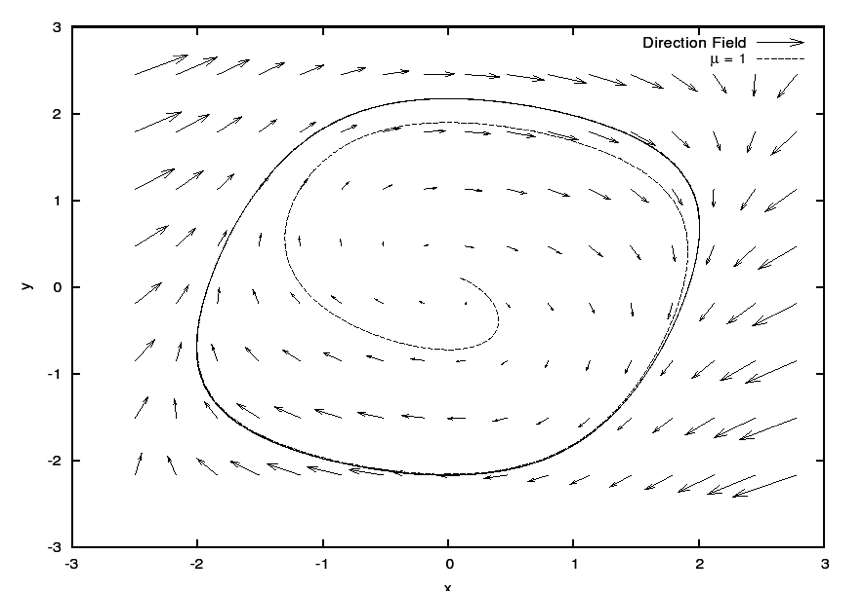
\includegraphics[scale=1]{dynamic_flow.png}
    \caption{连续时间动力学系统的相图}
    \label{fig:pha_spa}
\end{figure}
其中,我们称由所有维度的状态变量$\{x_1,x_2,\cdots,x_n\}$所张成的空间称为\textbf{相空间}。

对于一般的离散时间的动力学方程,我们可以用离散动力学方程\eqref{equ:map_dyna_sys}来描述:
\begin{equation}
    \begin{cases}
        \begin{aligned}
            x_1^{p+1} &= f_1(x_1^p,x_2^p,\cdots,x_n^p)\\
            x_2^{p+1} &= f_2(x_1^p,x_2^p,\cdots,x_n^p)\\
            \cdots &= \cdots \\
            x_n^{p+1} &= f_n(x_1^p,x_2^p,\cdots,x_n^p)
        \end{aligned}
    \end{cases}\label{equ:map_dyna_sys}
\end{equation}
其中$p\in \mathbb{N}$表示离散系统的迭代次数,即离散的时间指标。

\subsection{线性动力学系统}
在物理学中,我们比较熟悉的系统很多都是用线性方程描述动力学规律,即所谓的线性系统。线性方程很容易求解并且具有一些很简单的特性(如叠加原理)。在\eqref{equ:ode_dyna_sys}中,若$f_i(i=1,2,\cdots,n)$均为各自变量的线性函数,则我们的动力学系统即为一线性系统。连续时间线性系统可以用矩阵表示:
\begin{equation}
    \dot{x}=Ax
\end{equation}
其中$x$表示由所有状态变量构成的列向量,$A$为$n\times n$的矩阵($A_{ij}\in\mathbb{R}$)。

离散时间的线性动力学方程也可以用矩阵来表示:
\begin{equation}
    x_{n+1}=Ax_n
\end{equation}
其中$x$表示由所有状态变量构成的列向量,$A$为$n\times n$的矩阵($A_{ij}\in\mathbb{R}$),下标$n$表示系统的迭代次数,即离散的时间指标。

例如一个一维的连续时间线性系统$\dot{x}=3$,很容易求解其运动学方程为$x(t)=3t$,对应我们的一维匀速直线运动;再如系统$\dot{x}=-2x$,可以求解得到运动学方程为$x(t)=Ce^{-2t}$($C$为常数)。

\subsection{非线性动力学系统}
在实际中,许多物理现象乃至其他一些自然现象或者是社会现象毕竟是很复杂的,它们的动力学规律往往需要使用非线性方程表示。这些非线性方程除极少数外,一般都不存在解析解,但是它们却具有与线性方程解的不同的一些独特性质,所以非线性动力学需要一些其他的方法来研究其性质。若在\eqref{equ:ode_dyna_sys}中,若$f_i(i=1,2,\cdots,n)$有任意一个为自变量的非线性函数,则我们的动力学系统即为非线性系统。如一维弹性系统
\begin{equation}
    \ddot{x}+\omega^2x=0
\end{equation}
再如电子管振荡器中的范德波尔方程
\begin{equation}
    \ddot{x}+\alpha(x^2-1)\dot{x}+\omega^2x=0
\end{equation}

%由于在非线性系统中不易求得解析解,因此我们通常讨论非线性系统随时间的演化规律。在非线性系统中有一些特殊的性质,
我们将满足$\dot{x}=0$(连续时间系统)和$x_{n+1}=f(x_n)=x_n$(离散时间系统)的点$x^*$称为系统的\textbf{不动点}。在不动点处,系统状态变量不随时间发生变化。在连续时间系统中,我们将满足$T_{t^*}(x)=x$的轨道称为\textbf{周期轨道},周期为$t^*$,即粒子经过$t^*$时间后会回到起点;在离散时间系统中,我们将满足$x_{n+T}=x_n$的点称为\textbf{$T$周期点},周期为$T$,即粒子经过$T$次迭代又回到了起点。

\section{混沌系统}

混沌系统是指在一个确定性系统中,存在着貌似随机的不规则运动,其行为表现为不确定性、不可重复、不可预测,这就是混沌现象。混沌是非线性动力系统的固有特性,是非线性系统普遍存在的现象。混沌具有确定性、初值敏感性、不可预测性。

当系统作一般的规则运动时,无法避涨落所引起的初始条件的微小变化一般只引起运动状态的微小差别,即初始状态接近的轨道始终是接近的,从而人们可以对系统的运动作出预测。然而混沌却不然,它具有对初始条件的敏感依赖性,即初始条件的微小差别常常使轨道按指数形式分开。洛伦兹也曾戏称混沌运动对初始条件的敏感依赖性为“蝴蝶效应”。

对于一个实际系统,由于无法避免内部涨落和外部环境噪声等因素的影响,初始状态的微小差别难以避免,因此混沌对初始状态的这种敏感依赖性必然会导致运动的不确定性与随机性。由于这种随机性,混沌系统在有限的相空间中必然要有折叠,否则轨线就只能是封闭曲线(规则的周期运动)或延伸到无穷远(发散解)。对于连续时间动力学系统,混沌只可能出现在三维及以上的自治系统(微分方程中不显含时间)中。

洛伦兹系统就是1963年E.Lorenz研究模拟大气在地表受阳光加热时的情形时得到的混沌系统:
\begin{equation}
    \begin{cases}
        \dot{x}=\sigma(y-x)\\
        \dot{y}=x(\rho-z)-y\\
        \dot{z}=xy-\beta z
    \end{cases}\
\end{equation}
其中$x$、$y$、$z$分别为与对流强弱、对流引起的水平温差和垂直方向温差有关的变量,$\sigma$、$\rho$和$\beta$分别与普兰多(Prandtl)数、瑞利(Rayleigh)数和容器大小有关的参数,在用计算机求上式的数值解时,洛伦兹发现,在参数取适当值时,解具有非周期性与随机性。随后Henon和R\H ossler等人也得到了类似的结果。

关于混沌系统性质的讨论有很多,但是一般的方法直接观察系统的状态变量随时间的变化,即使观察时间很长,也不一定能看出规律。如果不对它作进一步的加工分析,很难了解其运动的性质和有关频谱成分等方面的信息,从而难以区分混沌和其他形式的震荡。当运动很复杂时,相空间中的轨迹可能是混乱一片甚至是充满某一区域而看不出什么规律。

为了研究复杂的非线性系统特别是混沌系统,通常有以下几种方法来进一步分析各种运动的特征。\textbf{频闪采样法}每隔一定时间观察轨迹上的代表点(采样点),这样,原来在相空间的连续运动就被一系列离散点$P_0$、$P_1$、
$P_2$、$\cdots$所代表,不同类型的运动可得到不同形态的采样结果,可以由此来分析其运动的性质。\textbf{庞加莱截面法}在多维相空间$\{x_1,x_2,\cdots,x_n\}$中选取一截面$f(x_i)=0$(此截面称为庞加莱截面),观察运动轨迹与此截面的截点(称为庞加莱点),则原来相空间的连续运动就被就被这些离散点$P_0$、$P_1$、
$P_2$、$\cdots$之间的映像所表示。\textbf{相空间重构法}选取一时间延迟量$T$,取$x(t)$、$x(t+T)$、$x(t+2T)$、$\cdots$、$x(t+mT)$为坐标画m维轨线,这样m个维度的变量随时间的变化隐含着整个系统的动力学规律,例如当相空间维度很高时,我们可以取$m=3$来重构高维的相空间,而三维的相空间我们则可以用图来形象化的描述。\textbf{功率谱法}是指任意函数都可以展开为一组基函数的线性组合,在物理中可理解为基频和一系列谐频的叠加,我们便可从频域分析原系统的动力学特征。



\section{Koopman算符}
Koopman算符由B.O.Koopman于1931年引入,它作用在某个函数上,描述了函数的演化。若将系统的特性数据演化视为函数的演化,我们即可以用Koopman算符分析系统的特征。现实中的许多系统,由于其动力学的复杂性而难以用较准确的动力学方程来近似描述,而只能得到通过实验或观测得到的系统特征数据。我们希望利用系统的特征数据,通过Koopman算符得到系统的动力学特征。

\subsection{Koopman算符的定义}
对于离散时间动力学系统,设对于相空间$\mathbf{P}$上的任意一点$x_p\in \mathbf{P}$,有$x_{p+1}=T(x_p)$。其中$p$为迭代次数,$T$描述了相空间的迭代规律。定义作用在相空间函数$f(x)$上的Koopman算符$U$, 使得:
\begin{equation}
    Uf(x)=f(T(x))
\end{equation}

对于连续时间动力学系统,设对于相空间$\mathbf{P}$上的任意一点$x_p\in \mathbf{P}$,有$x_t=T(x_0)$。其中下标$t$为时间,$T$描述了相空间随时间的演化规律。定义作用在相空间函数$f(x)$上的Koopman算符$U_t$,使得:
\begin{equation}
    U_tf(x)=f(T_t(x))
\end{equation} 

其中$f(x)$为定义在相空间上的任意可观测函数,如粒子的坐标、动量、浓度、概率密度等等。

给定$f(x)$,若令函数$\tilde{f}(x)=f(T(x))$,则Koopman算符可以描述函数的演化
\begin{equation}
    \begin{aligned}
        Uf(x)=f(T(x))=\tilde{f}(x)       &,&\text{(离散时间系统)}\\
        U_tf(x)=f(T_t(x))=\tilde{f}_t(x) &,&\text{(连续时间系统)}
    \end{aligned}
\end{equation}

例如,对于一个一维线性动力学方程
\begin{equation}
    \dot{x}=-2x
\end{equation}
其运动学方程$x(t)=x(0)e^{-2t}$,因此我们可以将其描述为
\begin{equation}
    T_t(x)=xe^{-2t}
\end{equation}
设我们有一在相空间的可观测函数
\begin{equation}
    f(x)=x^2
\end{equation}
若用Koopman算符作用在该函数上,我们可以得到
\begin{equation}
    U_tf(x)=f(T_t(x))=f(xe^{-2t})=x^2e^{-4t}=\tilde{f}(x)
\end{equation}
即Koopman算符作用在函数上,描述了函数的演化
\begin{equation}
    \begin{aligned}
        x^2 \stackrel{U_t}{\longrightarrow} x^2e^{-4t} \\
        f(x) \stackrel{U_t}{\longrightarrow} \tilde{f}(x)
    \end{aligned}
\end{equation}

Koopman算符$U$是无穷维的线性算符,即:
\begin{equation}
    U(\alpha f_1(x)+\beta f_2(x))=\alpha Ug_1(x)+\beta Ug_2(x)
\end{equation}
设有一个函数$f(x)$,我们将其分解到一组函数上$g_i(x)$($i=1,2,\cdots,n$)
\begin{equation}
    f(x)=\sum_{i=1}^n\alpha_ig_i(x)
\end{equation}
则Koopman算符可以描述为
\begin{equation}
    Uf(x)=U\sum_{i=1}^n\alpha_ig_i(x)=\sum_{i=1}^n\alpha_iUg_i(x)=\sum_{i=1}^n\alpha_ig_i(T(x))
\end{equation}
即一个复杂函数的演化规律可以描述为一组简单函数演化规律的线性叠加。

\subsection{Koopman算符的本征值与本征函数}
Koopman算符$U$是一个线性算符,可以对其进行谱分解。设有一复数$\lambda$和一复标量函数$\phi(x)$,使得
\begin{equation}
    U\phi(x)=\phi(T(x))=\lambda\phi(x)
\end{equation}
则称$\lambda$为Koopman算符的\textbf{本征值},$\phi(x)$为Koopman算符的\textbf{本征函数}。

Koopman算符的本征值和本征函数具有以下性质:

\textbf{性质1}:若$\phi_1(x)$,$\phi_2(x)$分别是Koopman算符U对应于$\lambda$的本征函数,则$\psi(x)=\alpha\phi_1(x)+\beta\phi_2(x)$也是U的本征函数,对应本征值为$\lambda$:
\begin{equation}
    U\psi(x)=\psi(T(x))=\alpha\phi_1(T(x))+\beta\phi_2(T(x))=\alpha\lambda\phi_1(x)+\beta
    \lambda\phi_2(x)=\lambda\psi(x)
\end{equation}

\textbf{性质2}:若$\phi_1(x)$,$\phi_2(x)$分别是Koopman算符$U$相应于本征值$\lambda_1$,$\lambda_2$的本征函数,则$\psi(x)=\phi_1(x)\phi_2(x)$也是$U$的本征函数,相应本征值为$λ_1λ_2$: 
\begin{equation}
U\psi(x)=\psi(T(x))=\phi_1(T(x))\phi_2(T(x))=\lambda_1\lambda_2\phi_1(x)\phi_2(x)=\lambda_1\lambda_2\psi(x)
\end{equation}

特别的,若$\phi(x)$是Koopman算符$U$相应于本征值$\lambda$的本征函数,则$\phi^n(x)$也是$U$的本征函数,相应的本征值为$\lambda^n$:
\begin{equation}
    U\phi^n(x)=(\phi(T(x)))^n=(\lambda\phi(x))^n=λ^n\phi^n(x)
\end{equation}

本征函数$\phi(x)$是一个在相空间上特殊的可观测函数,若将其在一组函数空间$\{g_1(x),g_2(x),\cdots,g_m(x)\}$中表示
\begin{equation}
    \phi(x)=\sum_{i=1}^m\alpha_ig_i(x)
\end{equation}
则Koopman算符描述本征函数$\phi(x)$的演化规律可以用一组基函数的演化规律来描述:
\begin{equation}
    \begin{aligned}
        U\phi(x)&=\sum_{i=1}^m\alpha_iUg_i(x)=\sum_{i=1}^m\alpha_ig_i(T(x))\\
        U\phi(x)&=\lambda\phi(x)=\sum_{i=1}^m\lambda\alpha_ig_i(x)
    \end{aligned}
\end{equation}

\subsection{Koopman算符的本征函数与相空间划分}

在动力学系统中,Koopman算符的本征值与本征函数有着特殊的含义。根据本征函数的定义,我们有
\begin{equation}
    \begin{aligned}
        \phi(x_p)=  &=U\phi(x_{p-1})=\lambda\phi(x_{p-1})\\
                    &=\lambda U\phi(x_{p-2})=\lambda^2\phi(x_{p-2})\\
                    &\cdots\\
                    &=\lambda^{n-1}U\phi(x_0)=\lambda^n\phi(x_0)
    \end{aligned}
\end{equation}
其中$p$为时间因子,我们可以看到,Koopman算符的本征函数值随着时间的演化呈$1/\lambda$倍变化,这反映了一种特殊的函数演化规律,而这个特殊的函数就是我们的Koopman算符的本征函数。相较于无规则的混沌演化,这种有规律的演化则更容易观察研究,而由于本征函数$\phi(x)$的特殊性,其必然反映了某种相空间的性质。因此,探究Koopman算符的本征函数的意义就变得尤为重要。

特别的,当$\lambda=1$时,则本征函数$\phi(x_p)=\phi(x_{p-1})=\cdots=\phi(x_{p-0})$($p\in \mathbb{Z}$为时间指标),此时本征函数不随时间发生变化,即$\phi(x)=C$($C$为常数),这与动力学系统中的守恒量相对应。例如在能量守恒定律中,就对应一个能量函数不随时间发生变化$E(x_1,\dot{x}_1,x_2,\dot{x}_2,\cdots,x_n,\dot{x}_n,t)=C$,亦可反推该函数是Koopman算符的本征函数。

当$|\lambda|=1$时(即$\lambda=e^{i\theta}$),则本征函数$|\phi(x_p)|=|\phi(x_{p-1})|=\cdots=|\phi(x_{p-0})|$($p\in \mathbb{Z}$为时间指标),此时本征函数的模不随时间发生变化(而相位在发生变化),这也对应了动力学系统中的一种守恒量。例如在匀速圆周运动中的速度矢量。

此外,在动力学系统中,周期轨道也反映了一种守恒量,Koopman算符的本征函数也与周期轨道有着密切的联系。

对于一个复杂的动力学系统,我们往往难以刻画其整体的动力学演化规律,因为许多系统的相空间在不同区域有着不同的性质。但若我们能够将动力学系统的相空间划分为多个区域,而每个区域的动力学系统有着相似的规律,我们便可以按区域描述相空间的演化规律。而相空间的划分又有着多种角度,我们可以从不同的角度对相空间进行划分,从而更具体的描述相空间的演化规律。

Koopman算符的本征值为我们提供了一个划分相空间的思路。对于Koopman算符谱中$|\lambda|=1$的本征值对应的本征函数,计算相空间中所有点的本征函数值,则本征函数值的模相同的点属于一个不变集。不变集中对应动力学系统的守恒量。若能通过这些不变集将相空间进行划分,我们便能实现对相空间运动模式的分块描述。因此我们可以求得Koopman算符的本征函数,并通过Koopman算符的本征函数实现对相空间的划分。通过多个本征函数从不同角度对相空间的划分,我们便可以更具体的刻画相空间的性质。


\subsection{Koopman谱分析与动力学模式}\label{section:Koop_dyna}

由于Koopman算符本征函数对相空间划分的重要性,我们将通过数值计算求得Koopman算符的本征函数。Koopman算符作用在函数上,描述了函数的演化规律。为了能够精确的描述一个本征函数,我们可以选取一组基函数$g_1(x),g_2(x),\cdots,g_m(x)$,$x\in \mathbb{R}$,其张成了一个函数空间,对于在该函数空间的任意函数$f(x)$,我们都可以表示为
\begin{equation}
    f(x)=\sum_{i=1}^m\alpha_ig_i(x)
\end{equation}
若我们能描述该函数空间内所有基函数的演化,则可以在该函数空间中求得我们的本征函数$\phi(x)$。
\begin{equation}
    Ug_i(x)=g_i(T(x))=\tilde{g}_i(x)
\end{equation}

为了得到Koopman算符的本征函数,我们需要构造演化前与演化后的数据,通常采用构造数据矩阵的方式,设某$p$时刻的数据为$\{x_{p_1},x_{p_2},\cdots,x_{p_n}\}$,$x_i\in \mathbb{R}^n$,当时刻为$p+1$时,数据演化为$\{x_{p_1+1},x_{p_2+1},\cdots,x_{p_n+1}\}$,$x_i\in \mathbb{R}^n$,在选取的基函数${g_i(x)}$,$i=1,2,\cdots,m$下,利用已知数据点将m个基函数及演化后的函数表示为在$\{x_{p_1},x_{p_2},\cdots,x_{p_n}\}$(称之为“演化格点”)下的列向量,从而构成两个$n\times m$的数据矩阵:
\begin{equation}
    \begin{aligned}
        K=(g_1(x_p),g_2(x_p),\cdots,g_m(x_p))=
        \begin{pmatrix}
        g_1(x_{p_1}) & g_2(x_{p_1}) & \cdots & g_m(x_{p_1}) \\
        g_1(x_{p_2}) & g_2(x_{p_2}) & \cdots & g_m(x_{p_2}) \\
        \vdots       & \vdots       & \ddots & \vdots \\
        g_1(x_{p_n}) & g_2(x_{p_n}) & \cdots & g_m(x_{p_n})
        \end{pmatrix}
    \end{aligned}
\end{equation}
\begin{equation}
    \begin{aligned}
    L=&(g_1(x_{p+1}),g_2(x_{p+1}),\cdots,g_m(x_{p+1}))\\
    =&(\tilde{g}_1(x),\tilde{g}_2(x),\cdots,\tilde{g}_m(x))=
        \begin{pmatrix}
        g_1(x_{p_1+1}) & g_2(x_{p_1+1}) & \cdots & g_m(x_{p_1+1}) \\
        g_1(x_{p_2+1}) & g_2(x_{p_2+1}) & \cdots & g_m(x_{p_2+1}) \\
        \vdots         & \vdots         & \ddots & \vdots \\
        g_1(x_{p_n+1}) & g_2(x_{p_n+1}) & \cdots & g_m(x_{p_n+1})
        \end{pmatrix}
    \end{aligned}
\end{equation}

其中$K$我们称为演化前矩阵,$L$称为演化后矩阵,$K$、$L$的每一列为相空间在一组点在某个基函数上的取值,当相空间的点数足够多时,可以视矩阵的每一列为一个基函数的离散数据表示,$K$、$L$则可以看作是多个基函数的组合,分别表示演化前的基函数和演化后的基函数,而演化后的基函数又可以看作一个新的函数,视为Koopman算符作用在基函数上得到。于是$K$、$L$之间的关系可由Koopman算符表示
\begin{equation}
    UK=L
\end{equation}
Koopman算符的矩阵表示可由上式确定,因此我们可以通过上式求得Koopman算符的矩阵表示,进一步求得Koopman算符的本征值与本征函数。

% 以Logistic映射为例,我们介绍Koopman分析的算法实现与具体步骤,不失一般性,我们取特定的参数$\gamma=4$,此时Logistic映射表现为混沌状态,此时Logistic映射的动力学方程可以描述为
% \begin{equation}
%     x_{n+1}=f(x_n)=4x_n(1-x_n),x_n\in [0,1],n=1,2,3,\cdots
% \end{equation}

% 该系统为一维系统,相空间范围为$[0,1]$,该系统存在两个不动点:$0$和$3/4$。我们首先根据该映射方程产生一组迭代数据,设我们产生的迭代数据的数量为$n+1$。则每个数据点可以表示为$x_i,i=1,2,\cdots,n+1$,为了得到“演化前数据”和“演化后数据”,我们将这组迭代产生的数据构造为$\{x_1,x_2,\cdots,x_n\}$与$\{x_2,x_3,\cdots,x_{n+1}\}$,并根据这两组数据构造出数据矩阵$K$与$L$。

在构造矩阵$K$与$L$时,我们需要选定一组基函数${g_i(x)},i=1,2,\cdots,m$,基函数的选取对我们计算本征函数的结果至关重要,于是我们将从多个角度讨论基函数的选取对本征函数的影响。基函数的选取至关重要,为了能较好的表示出Koopman算符的本征函数,需要一组较完备的基函数作为算符作用的可观测量,可以选取Gauss基函数、Fourier基函数、Legendre基函数。然而上述基函数只有在数量趋于无穷时才具有完备性,我们希望基函数的数量足够多,然而为了相空间的数据点能够较好的表示每个基函数,基函数的数量又不宜超过演化格点的数量,此外考虑到计算量的因素,我们只能将基函数的数量设为某个有限值。此外由于相空间粒子分布的不均匀性,我们还可以取不同分布的基函数。总之,基函数的选取有多重形式,而基函数的选取会影响到本征函数的计算,因此基函数的选取至关重要。

在选取合适的基函数与构造数据矩阵K与L后,我们即可以根据$UK=L$计算求得Koopman算符的矩阵表示以及本征值与本征函数,通常我们会得到n个本征值与本征函数,而在这些本征值中,我们比较关心的是本征值(或者本征值的模)接近1的本征函数,因为本征值为1的本征函数反映了相空间中一条随时间演化不变的轨道,这种轨道即是系统的一个关键特征,而由于我们的数值计算误差,因此我们将选取接近1的本征值对应的本征函数。

Koopman算符对相空间的划分可以通过混沌系统的已知特性来得到验证,如在Logistic映射中有两个不动点,而我们得到的本征函数图像恰好在不动点以及不动点的原像处得到了本征函数的极值点,说明了本征函数能够体现系统的动力学特征;此外,我们还可以通过验证动力学系统的周期点与周期轨道等特征,对比Koopman算符的本征函数,以此观察Koopman算符分析动力学系统的可行性。

Koopman算符理论上能够区分相空间的不同区域的性质,对于具有噪声的数据和涨落的演化规律,Koopman算符同样可以通过控制函数空间的精细度来对相空间进行粗细粒度的划分,因此Koopman算符具有鲁棒性:即使我们的演化有噪声的影响,如探究噪声中常见的高斯白噪声,我们同样可以对相空间进行粗粒度的划分。这在我们探究动力学系统中的演化规律中尤为重要。

\subsection{动力学系统的符号动力学与“边界点”}

符号动力学起源于动力系统的抽象拓扑理论的研究,并从20世纪60年代起逐渐在应用于一维映射的研究过程中得到发展和完善。符号动力学是研究符号动力系统的学科,这种系统的状态均可表示为有限个符号的无穷序列,而由任一状态点引出的运动轨道可由表示该状态的无穷序列通过简单的移位规则来确定。许多复杂动态系统均可经过变换等价于这类系统,从而可通过对比较简单的符号动力系统的分析来研究一般动力系统的行为。这种方法特别在混沌等复杂行为研究中占有重要地位。符号动力系统在其他领域也有广泛的应用。例如研究离散事件动态系统控制问题的代数方法就与符号动力学有密切的联系。

符号动力学是实际动力系统的抽象和概括。对于一个相空间的离散动力学系统,我们可以依据不同的符号将相空间的不同区域命名,如使用符号“0”和符号“1”来讲相空间划分为两个区域。通过相空间的演化,又可以继续用有限个符号来更加细致的划分相空间。理论上相空间中的每个点都可以用一个无穷的符号序列与之对应。当传统的微分理论难以对动力学系统分析时,我们可以使用粗粒度的符号动力学来研究动力学系统的性质。即使一般的数值方法行不通,符号动力学仍可以对系统进行定性分析。

Logistic映射就是一个可用符号动力学很好描述的典型,Logistic映射的动力学方程
\begin{equation}
    x_{n+1}=f(x_n)=\gamma x_n (1-x_n ),x_n∈[0,1],\ n=1,2,3,\cdots
\end{equation}
这里我们取$\gamma=4$,Logistic映射的迭代过程使它成为一个经典的混沌系统,符号动力系统也被视为混沌系统的原型,进而还可将符号动力系统的运动特征作为混沌的描述并成为混沌的一种严格的数学定义。Logistic映射的相图与符号动力学的划分可由下图表示:
\begin{figure}
	\centering
	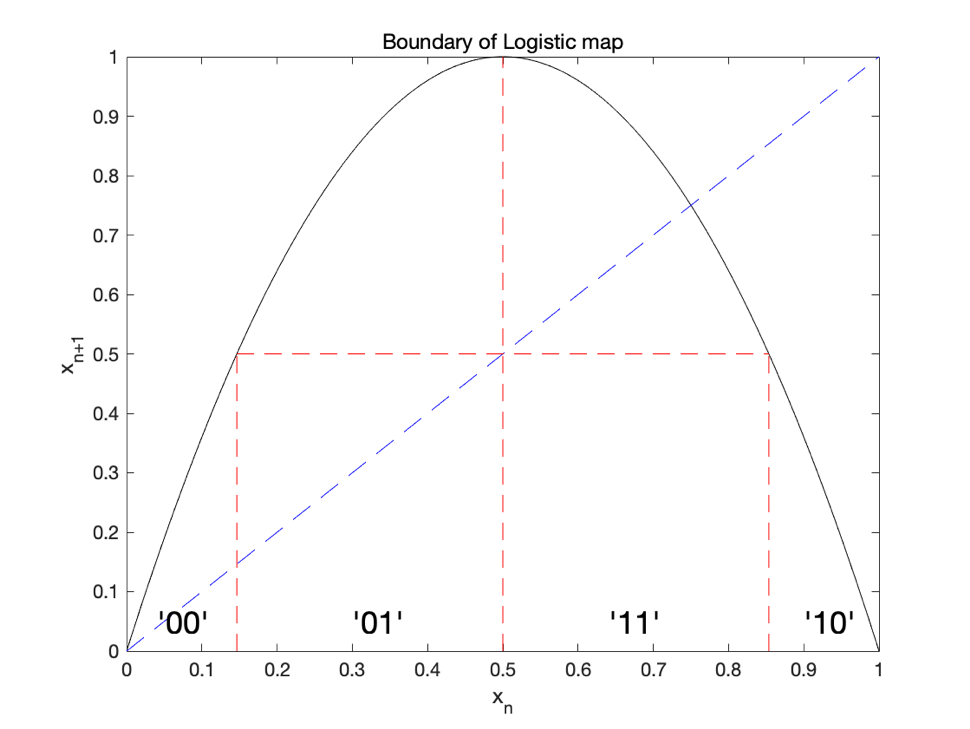
\includegraphics[scale=0.6]{logistic_symbolic.png}
    \caption{Logistic映射的符号动力学划分}
    \label{fig:logi_symb}
\end{figure}
Logistic映射的动力学过程可以看作是在一维相空间上的拉伸再折叠的过程,在折叠的临界点处$x=\frac{1}{2}$我们将其作为一个“临界点”,在临界点的两边我们分别标记区域为“0”和"1"。而在"0"区域的相空间$x\in [0,\frac{1}{2}]$中,其下一步演化的位置即存在演化为"0"的点,也存在演化为"1"的点。这样,我们可以根据该区域一次演化的结果进行更进一步的划分,则“0”区域的相空间又可以划分为"00"和"01"的相空间;同理,“1”区域的相空间可以划分为"11"和"10"的相空间。若将二次演化乃至多次演化作为划分符号动力学相空间的评判标准,则我们可以用符号动力学标记任意精度的相空间区域。特别的,在极限情况下,当我们演化的次数足够多时,我们可以对相空间的每个足够小的区域都划分出来,即相空间的每个点都对应一组无穷符号序列。

在符号动力学中,一个最关键的问题就是如何寻找“边界点”,\text{边界点}是指在符号动力学中可以划分相空间不同区域的临界点,如在Logistic映射中,$x=\frac{1}{2}$就是一个“边界点”,根据其演化我们还可以找到一次演化的边界点$x=\frac{1}{2}\pm\frac{\sqrt{2}}{4}$,以此类推。所以,若能找到系统的“边界点”,便可以通过符号动力学对其相空间进行划分。

Koopman算符的本征函数能够划分相空间区域的不同性质,而符号动力学的边界点也是反映了相空间区域的划分。当相空间的性质足够简单时,我们对其划分的标准就更单一。于是我们可以认为,此时Koopman算符的本征函数对相空间的划分恰好就是反映了符号动力学中的“边界点”对相空间的划分。我们将在后面的例子中继续探究这两者之间的对应关系。Koopman算符的本征函数恰能反映符号动力学的“边界点”,这也为我们寻找符号动力学的“边界点”提供了一个有效的方法。

\subsection{Koopman算符的函数空间}
% Rectangle Gauss Fourier Legendre
\subsubsection{正交完备基函数簇}
在\ref{section:Koop_dyna}节的讨论中,我们要选择一组基函数${g_i(x)},i=1,2,\cdots,m$来构造数据矩阵$K$与$L$,这里的基函数即限定了我们的函数空间,我们的本征函数由这组基函数来描述,因此,如何选择合适的基函数成为了一个至关重要的问题。

为了较好的表示出Koopman算符的本征函数,我们应选取一组正交完备的基函数来描述本征函数。完备性使得在此函数空间的任意函数都能且仅能得到一组唯一的线性组合。正交性使得基函数之间互不依赖。一般的,我们将定义在区间$[a,b]$上的一组基函数${g_i(x)}$的正交归一性用以下函数的内积来表示:
\begin{equation}
    <g_i,g_j>=\int_a^b{g_i(x)g_j(x)}dx=\delta_{ij}=
    \begin{cases}
        1,\ (i=j)\\
        0,\ (i\neq j)
    \end{cases}
\end{equation}

举一些基函数的例子。对于一维系统,设相空间为$x\in [0,1]$,我们在这个相空间范围内选取一组基函数${g_i(x)},i=1,2,\cdots,m$。考虑到正交性,对于最简单的一个例子就是矩形窗基函数:
\begin{equation}
    g_i(x)=
    \begin{cases}
        \sqrt{m},\ &(\dfrac{i-1}{m}\leq x<\dfrac{i}{m})\\
        0,\ &(x为其他)
    \end{cases},\ i=1,2,\cdots,m
\end{equation}
矩形窗基函数是一个局域化的函数,其结构足够简单,其所描述的函数空间总是能按照本征函数值区分相空间。

矩形窗基函数的每个函数之间没有任何冗余信息,这样很多函数都没有起到描述相空间的作用,为此我们可以将函数取为一组近似局域化的高斯基函数:
\begin{equation}
    g_i(x)=Cexp\left(-\dfrac{(x-x_i)^2}{2d_j^2}\right), \ x_i=\frac{i}{m}-\frac{1}{2m},\ i=1,2,\cdots,m
\end{equation}
其中C为高斯函数的归一化常数$C=\frac{1}{\sqrt{\sqrt{\pi}\sigma}}$。高斯基函数满足近似正交性,是一组近似局域性的全局基函数,每个函数都定义在整个相空间上,其形状类似一“波包”。其中有两个参数:波包中心$x_i$和波包宽度$d_j$。波包中心$x_i$表示高斯波包的中心位置,其选取通常应遍布大部分相空间,为了减少边界效应,一般情况下我们选取$x_i=\frac{i}{m}-\frac{1}{2m}$;波包宽度$d_j$描述高斯波包衰减到$\sqrt{\frac{1}{e}}$的距离,其选取应综合考虑相空间粒子的一步演化距离和函数之间的重叠,一般情况下我们选取$d_j=\frac{1}{2m}$。计算表明,使用高斯基函数可以得到较为清晰的动力学系统的相空间划分。

除了上述两个局域化的基函数,我们还可以考虑非局域化的基函数。如定义在$x\in [0,1]$上的傅里叶基函数
\begin{equation}
    g_k(x)=e^{ik(2\pi)x},\ k=-m,-(m-1),\cdots,m-1,m
\end{equation}
傅里叶基函数描述了每个频率的重要程度。再如多项式基函数
\begin{equation}
    g_i(x)=x^i,\ i=0,1,\cdots,m
\end{equation}
和其处于同一函数空间的定义在$x\in [-1,1]$上的勒让德基函数
\begin{equation}
    g_i(x)=\sqrt{\dfrac{2k+1}{2}}P_i(x),\ k=0,1,\cdots,m
\end{equation}

下图绘制了一维矩形窗基函数、高斯基函数、傅里叶基函数和勒让德基函数的图像
\begin{figure}
	\centering
	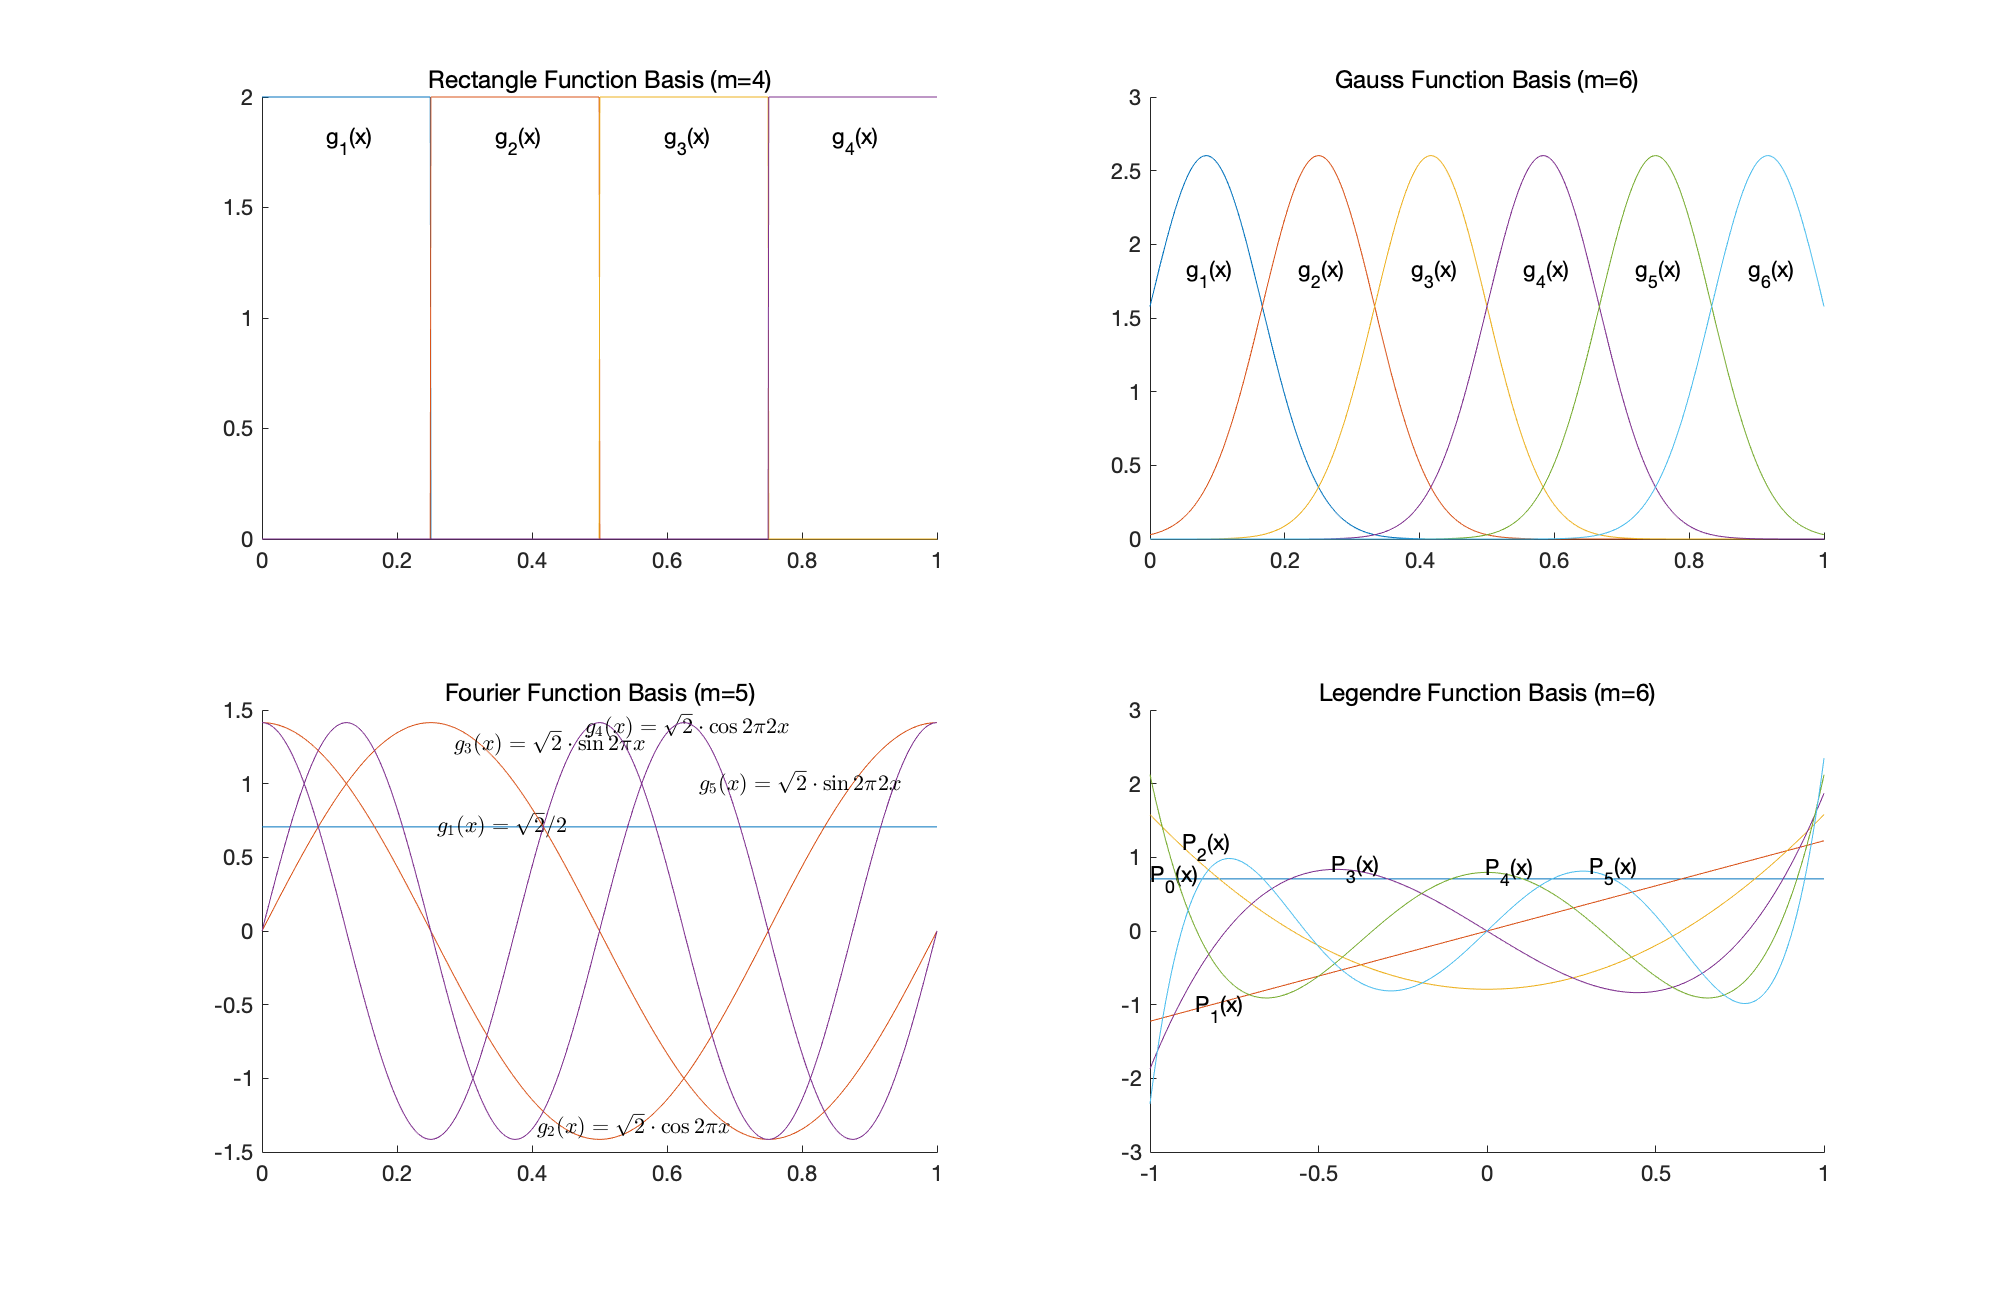
\includegraphics[scale=0.2]{function_basis}
    \caption{矩形窗、高斯、傅里叶、勒让德基函数图像}
    \label{fig:func_bas}
\end{figure}

对于高维系统,亦可以将上述方程扩展,如高维傅里叶基函数与高维高斯基函数。对于任意$n$位动力学系统,我们总是可以构造一组$n$维函数空间,将本征函数在此$n$维函数空间描述,我们便可以更准确的描述本征函数,从而对我们的相空间进行划分。

\subsubsection{自然演化的函数空间}

在\ref{section:Koop_dyna}节中,我们在动力学系统中可以选取一组合适的基函数,并将本征函数在此基函数中进行描述。这里考虑另一种取基函数的方法:自然演化的函数空间。对于在相空间$\mathbb{p}$中的系统状态变量$x_i$,我们取一个初始状态$x_i$,并将其进行$n$次演化,得到一组随时间演化的状态变量$(x_i,x_{i+1},\cdots,x_{n+i-1})^T$,这组状态变量也可以看做是相空间的一个$n$维函数,只不过其是由自然演化得到的。对于这样的一个基函数$g_i(x)=(x_i,x_{i+1},\cdots,x_{n+i-1})^T$,我们将Koopman算符作用在$g_1(x)$上可以得到
\begin{equation}
    Ug_i(x)=U(x_i,x_{i+1},\cdots,x_{n+i-1})^T=(x_{i+1},x_{i+2},\cdots,x_{n+i})^T=g_{i+1}(x)
\end{equation}

我们连续的取$m$个这样的自然演化的基函数$g_i(x)=(x_i,x_{i+1},\cdots,x_{n+i-1})^T$,并利用自然演化的基函数构造数据矩阵$K$和$L$:
\begin{equation}
    K=\{g_1(x),g_2(x),\cdots,g_m(x)\}=
    \begin{pmatrix}
        x_1 & x_2 & \cdots & x_m \\
        x_2 & x_3 & \cdots & x_{m+1} \\
        \vdots         & \vdots         & \ddots & \vdots \\
        x_n & x_{n+1} & \cdots & x_{n+m-1}
    \end{pmatrix}
\end{equation}
\begin{equation}
    L=\{g_2(x),g_3(x),\cdots,g_{m+1}(x)\}=
    \begin{pmatrix}
        x_2 & x_3 & \cdots & x_{m+1} \\
        x_3 & x_4 & \cdots & x_{m+2} \\
        \vdots         & \vdots         & \ddots & \vdots \\
        x_{n+1} & x_{n+2} & \cdots & x_{n+m}
    \end{pmatrix}
\end{equation}
$K$、$L$的每一列为相空间在一个初始点上的演化,当演化次数$n$足够多时,我们可以用这组演化来表示一个描述相空间的自然函数,$K$、$L$可以看作是多个基函数的组合,分别表示演化前和演化后的自然函数。同样的,数据矩阵$K$、$L$之间的关系可由Koopman算符表示
\begin{equation}
    UK=L
\end{equation}

不同于\ref{section:Koop_dyna}节中我们构造的函数空间,自然演化的函数空间仅由系统的动力学演化得到,其更能反映动力学系统的本征行为。我们可进一步求出在自然演化的基函数中Koopman算符的本征函数并以此来划分相空间。



%% 本章参考文献
% \ifx\usechapbib\empty
% \nocite{BSTcontrol}
% \setcounter{NAT@ctr}{0}
% \bibliographystyle{buptgraduatethesis}
% \bibliography{references}
% \fi
